%%%%%%%%%%%%%%%%%%%%%%%%%%%%%%%%%%%%%%%%%
% Short Sectioned Assignment LaTeX Template Version 1.0 (5/5/12)
% This template has been downloaded from: http://www.LaTeXTemplates.com
% Original author:  Frits Wenneker (http://www.howtotex.com)
% License: CC BY-NC-SA 3.0 (http://creativecommons.org/licenses/by-nc-sa/3.0/)
%%%%%%%%%%%%%%%%%%%%%%%%%%%%%%%%%%%%%%%%%

%----------------------------------------------------------------------------------------
%	PACKAGES AND OTHER DOCUMENT CONFIGURATIONS
%----------------------------------------------------------------------------------------

\documentclass[paper=a4, fontsize=11pt]{scrartcl} % A4 paper and 11pt font size

% ---- Entrada y salida de texto -----

\usepackage[T1]{fontenc} % Use 8-bit encoding that has 256 glyphs
\usepackage[utf8]{inputenc}
%\usepackage{fourier} % Use the Adobe Utopia font for the document - comment this line to return to the LaTeX default

% ---- Idioma --------

\usepackage[spanish, es-tabla]{babel} % Selecciona el español para palabras introducidas automáticamente, p.ej. "septiembre" en la fecha y especifica que se use la palabra Tabla en vez de Cuadro

% ---- Otros paquetes ----

\usepackage{url} % ,href} %para incluir URLs e hipervínculos dentro del texto (aunque hay que instalar href)
\usepackage{amsmath,amsfonts,amsthm} % Math packages
%\usepackage{graphics,graphicx, floatrow} %para incluir imágenes y notas en las imágenes
\usepackage{graphics,graphicx, float} %para incluir imágenes y colocarlas
\usepackage{epstopdf}

% Para hacer tablas comlejas
%\usepackage{multirow}
%\usepackage{threeparttable}

%\usepackage{sectsty} % Allows customizing section commands
%\allsectionsfont{\centering \normalfont\scshape} % Make all sections centered, the default font and small caps

\usepackage{fancyhdr} % Custom headers and footers
\pagestyle{fancyplain} % Makes all pages in the document conform to the custom headers and footers
\fancyhead{} % No page header - if you want one, create it in the same way as the footers below
\fancyfoot[L]{} % Empty left footer
\fancyfoot[C]{} % Empty center footer
\fancyfoot[R]{\thepage} % Page numbering for right footer
\renewcommand{\headrulewidth}{0pt} % Remove header underlines
\renewcommand{\footrulewidth}{0pt} % Remove footer underlines
\setlength{\headheight}{13.6pt} % Customize the height of the header

\numberwithin{equation}{section} % Number equations within sections (i.e. 1.1, 1.2, 2.1, 2.2 instead of 1, 2, 3, 4)
\numberwithin{figure}{section} % Number figures within sections (i.e. 1.1, 1.2, 2.1, 2.2 instead of 1, 2, 3, 4)
\numberwithin{table}{section} % Number tables within sections (i.e. 1.1, 1.2, 2.1, 2.2 instead of 1, 2, 3, 4)

\setlength\parindent{0pt} % Removes all indentation from paragraphs - comment this line for an assignment with lots of text

\newcommand{\horrule}[1]{\rule{\linewidth}{#1}} % Create horizontal rule command with 1 argument of height


%----------------------------------------------------------------------------------------
%	TÍTULO Y DATOS DEL ALUMNO
%----------------------------------------------------------------------------------------

\title{	
\normalfont \normalsize 
\textsc{\textbf{Curso 2016-2017} \\ Grado en Ingeniería Informática \\ Universidad de Granada} \\ [25pt] % Your university, school and/or department name(s)
\horrule{0.5pt} \\[0.4cm] % Thin top horizontal rule
\huge Documentación práctica 2 TSI: \\Explorador basado en fronteras. \\ % The assignment title
\horrule{2pt} \\[0.5cm] % Thick bottom horizontal rule
}

\author{Carlos Manuel Sequí Sánchez} % Nombre y apellidos

\date{\normalsize\today} % Incluye la fecha actual

%----------------------------------------------------------------------------------------
% DOCUMENTO
%----------------------------------------------------------------------------------------

\begin{document}

\maketitle % Muestra el Título

\newpage %inserta un salto de página

\tableofcontents % para generar el índice de contenidos

\newpage




\section{Ejercicios planteados en ''EjerciciosMapeo1''}

\subsection{Giro de 360º}

Con el fin de reconocer/explorar los alrededores del robot implementamos este método. Su funcionamiento es simple, hacemos, mediante el uso de parámetros o atributos de ros, que la base gire sobre sí misma para reconocer su entorno y rellenar el mapa sobre el que está. \\

Para obtener mejores resultados nos basta con realizar dos vueltas completas, ya que con una sola vuelta no recoge información suficiente el sensor.\\

La velocidad angular la he puesto a 2*$\pi$. \\ 

Pseudocódigo:


\begin{algorithmic}[1]
	\While {TiempoDeGiro}
	\State{Girar sobre sí mismo}
	\EndWhile
\end{algorithmic}

\subsection{Rellenar obstáculos}

Método cuyo propósito es hacer que el robot no vaya hacia zonas donde hay obstáculos para evitar impactar contra alguno de estos.\\
Desde getmapCallBack llamamos a este método para cada una de las casillas que hay en la matriz que representa el mapa sobre el que se sitúa el robot (cmGlobal). Resumiendo un poco, el funcionamiento se basa en recorrer toda la matriz del mapa y, en cuanto encontramos una casilla obstáculo (con valor 100) hacemos que las casillas que se encuentran a su alrededor seas también obstáculos, concretamente 10 casillas hacia cada uno de los 4 lados de la casilla central (realizando cálculos son 10 casillas las que hay que modificar para cumplir ese metro cuadrado que se pide en el guión).\\ \\
Pseudocódigo:

\begin{algorithmic}[1]
	\For{cantidad de filas}
		\If{estamos dentro del límite de anchura}
			\For{cantidad de columnas}
				\If{estamos dentro del límite de altura.}
					\State{theGlobalCm[filaActual][columnaActual] = 100;}
				\EndIf
			\EndFor
		\EndIf
	\EndFor
\end{algorithmic}

\subsection{Etiquetar celdas frontera}

Este método se encarga de detectar los nodos frontera en el mapa, básicamente lo explora por completo (exploramos la matriz theGlobalCM) y, para cada una de las casillas de dicha matriz, en caso de que sea una casilla libre y además al menos una de sus casillas vecinas sea desconocida (cosa que sabemos gracias al método someNeighbour is unknown) pues la etiquetamos como casilla frontera, añadiéndola al vector "frontera" para que la base más tarde haga uso del método selectNode para seleccionar el nodo objetivo.\\

Pseudocódigo:


\begin{algorithmic}[1]
	\State{vaciarVectorFrontera();}
	\For{cantidad de filas}
		\For{cantidad de columnas}
			\If{casillaActual es vacía y además tiene vecino desconocido}
				\State{calcularCoordenadasReales();}
				\State{insertarCoordenadasEnVectorFrontera();}
			\EndIf
		\EndFor
	\EndFor
\end{algorithmic}


\subsection{Seleccionar nodo objetivo}

Para este método el criterio por el que he optado es ir escogiendo sucesivamente el nodo de la frontera que más lejano se encuentra a la posición actual de robot, con el fin de que explore la mayor parte del mapa en
un tiempo reducido, ya que en cada una de las "iteraciones" (entendiendo como iteración cada una de las veces que llega a un objetivo) se aumenta el tamaño de la distancia a recorrer entre nodos objetivos, cosa que hace que la base recorra cada vez más y más espacio.\\
En cuanto a código simplemente he ido recorriendo cada uno de los nodos del vector frontera con el fin de calcular sus distancias e ir actualizando el nodo con mayor distancia desde la posición actual de la base.\\

Pseudocódigo:

\begin{algorithmic}[1]
	\State{Dist = distancia máxima final}
	\For{cantidad de nodos en frontera}
	\State{dist2 = calcular distancia entre robot y el nodo actual}
	\If{dist2 > Dist}
	\State{actualizamos el nodo más lejano;}
	\State{Dist = dist2;}
	\EndIf
	\EndFor
\end{algorithmic}

\newpage

\section{Estrategia en caso de fallo}

En caso de fallo por parte del robot a la hora de comprobar si ha podido o no llegar al objetivo ("The base failed for some reason") he utilizado la estrategia de hacer que la base rote 4 veces con el fin de detectar sus alrededores de forma óptima y tras ello escoger un punto intermedio distinto al más lejano, es decir, en caso de fallo, hago la llamada a mi método calculaIntermedio(), el cual calcula el punto intermedio (en cuanto a distancia se refiere) entre el robot y el punto más lejano (¡Ojo! no calcula el punto intermedio en ruta desde la posición actual de la base HACIA el punto de la frontera mas lejano, sino otro punto de otra ruta que esta a la mitad de distancia de lo que estaba el punto más lejano en un principio). \\
En cuanto a la explicación del método que realiza este cálculo es simple: en un contenedor "set" de la STL de C++ almaceno pares de valores distancia-índice, de modo que el primer valor me indica la distancia entre la posición actual y el punto de la frontera que indica el segundo valor (índice). Como este contenedor se encarga solo de ordenar en orden creciente según el valor del primer atributo de cada par que es introducido, solo he de hacer un recorrido por el vector "frontera" para ir extrayendo su información en forma de pares (pair<distancia,indice>) e ir introduciéndolos en el contenedor set. De tal manera, una vez ordenados, solo he de indicar que el nodo intermedio es el que se encuentra en la posición intermedia del contenedor que he rellenado previamente. Con esto pretendo conseguir que, en caso de que la base no pueda ir hasta el nodo más lejano de la frontera por cualquier razón, intente ir al nodo que tiene a media distancia, incrementando así las posibilidades de acierto.\\


Pseudocódigo:

\begin{algorithmic}[1]
	\For{cantidad de elementos en la frontera}
		\State{calcular distancia al robot;}
		\State{almacenar distancia en pair;}
		\State{almacenar índice en pair;}
	\EndFor
	
	\State{nuevoNodoObjetivo = indice intermedio del set de pairs;}
\end{algorithmic}

\newpage

\section{Experimentos realizados}

Una vez implementados los cuatro ejercicios recomendados y mi propia estrategia me dispuse a realizar los dos experimentos indicados: 

\subsection{Corridor}

Primero el más sencillo, con un tiempo de 446.6 segundos como muestro a continuación, se recorre el mapa por completo sin ningún tipo de problemas y, cuando finaliza, la base vuelve al nodo origen. \\


Captura del final de la ejecución, donde se muestra el mapa descubierto al completo por la base: \\

\begin{figure}[H] %con el [H] le obligamos a situar aquí la figura
	\centering
	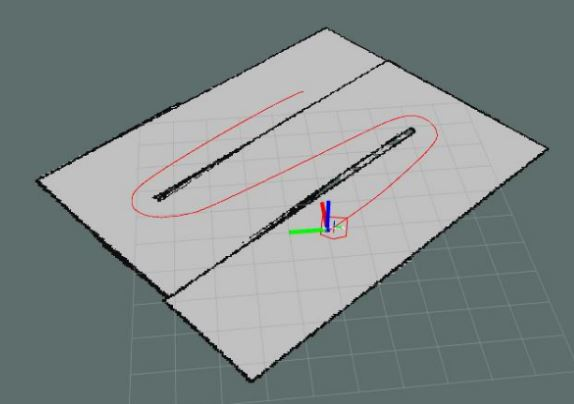
\includegraphics[scale=0.9]{1} 
\end{figure}

\newpage

\subsection{Willow garage}

Por último realizamos el experimento con el mapa complicado. Tras estar ejecutándose unos 30 minutos la base consiguió completar el mapa tal y como lo muestro en la siguiente figura (en azul señalo donde se encuentra el robot en el momento que tomé la captura).\\
He de decir que el robot durante la ejecución se choca varias veces y que además tarda un buen rato en recuperarse y continuar moviéndose por el mapa tras un golpe.
\\

\begin{figure}[H] %con el [H] le obligamos a situar aquí la figura
	\centering
	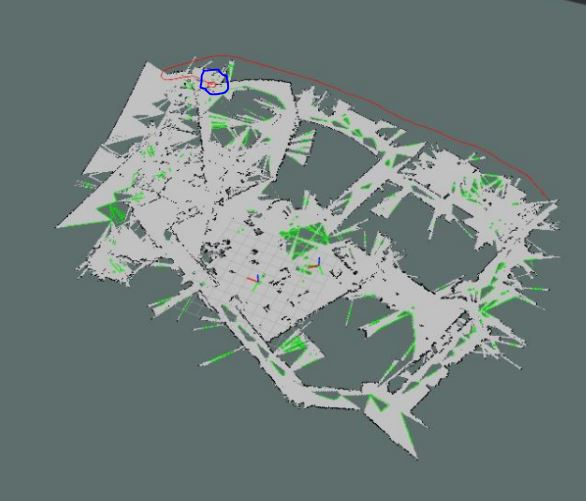
\includegraphics[scale=0.9]{3} 
\end{figure}


\newpage
%------------------------------------------------



\end{document}
